

\subsection{Results}\label{M1:results}
\subsubsection{Sanity checks}
Show and discuss the results.

\note{FIX Colors on omega plot. Should coincide with others}

\begin{figure}
    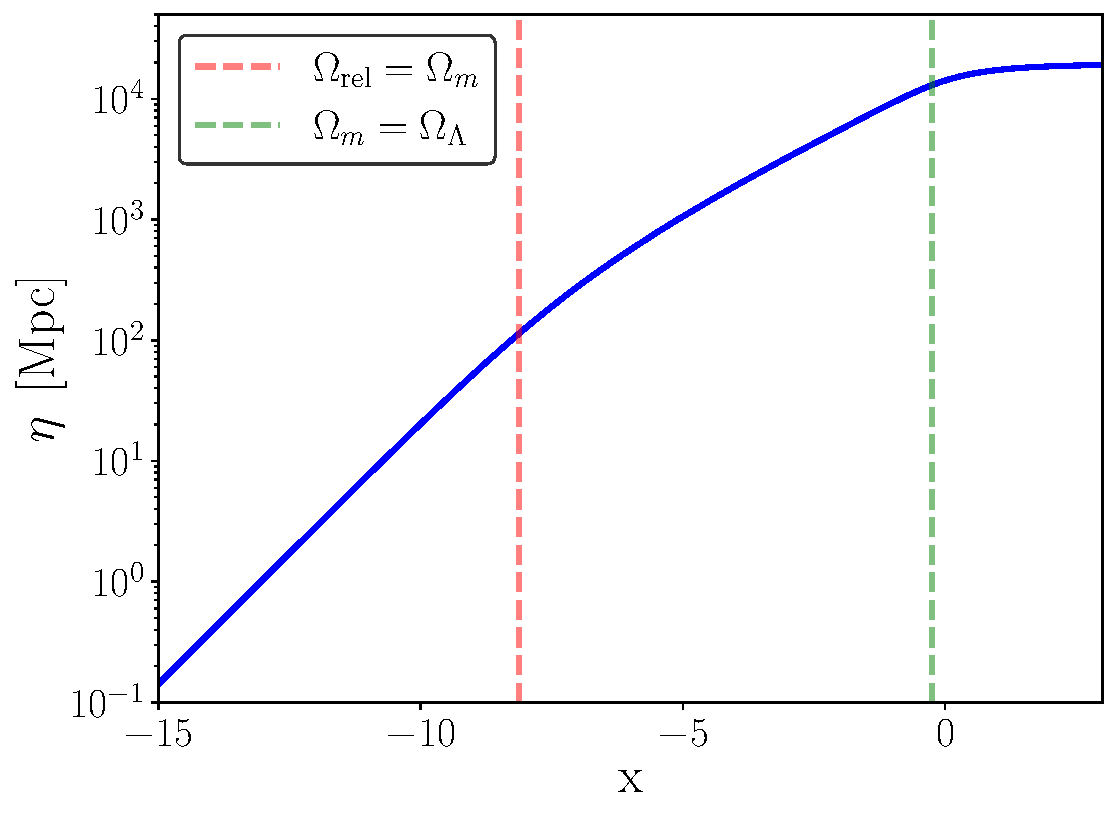
\includegraphics[width=\linewidth]{compare_eta.pdf}
    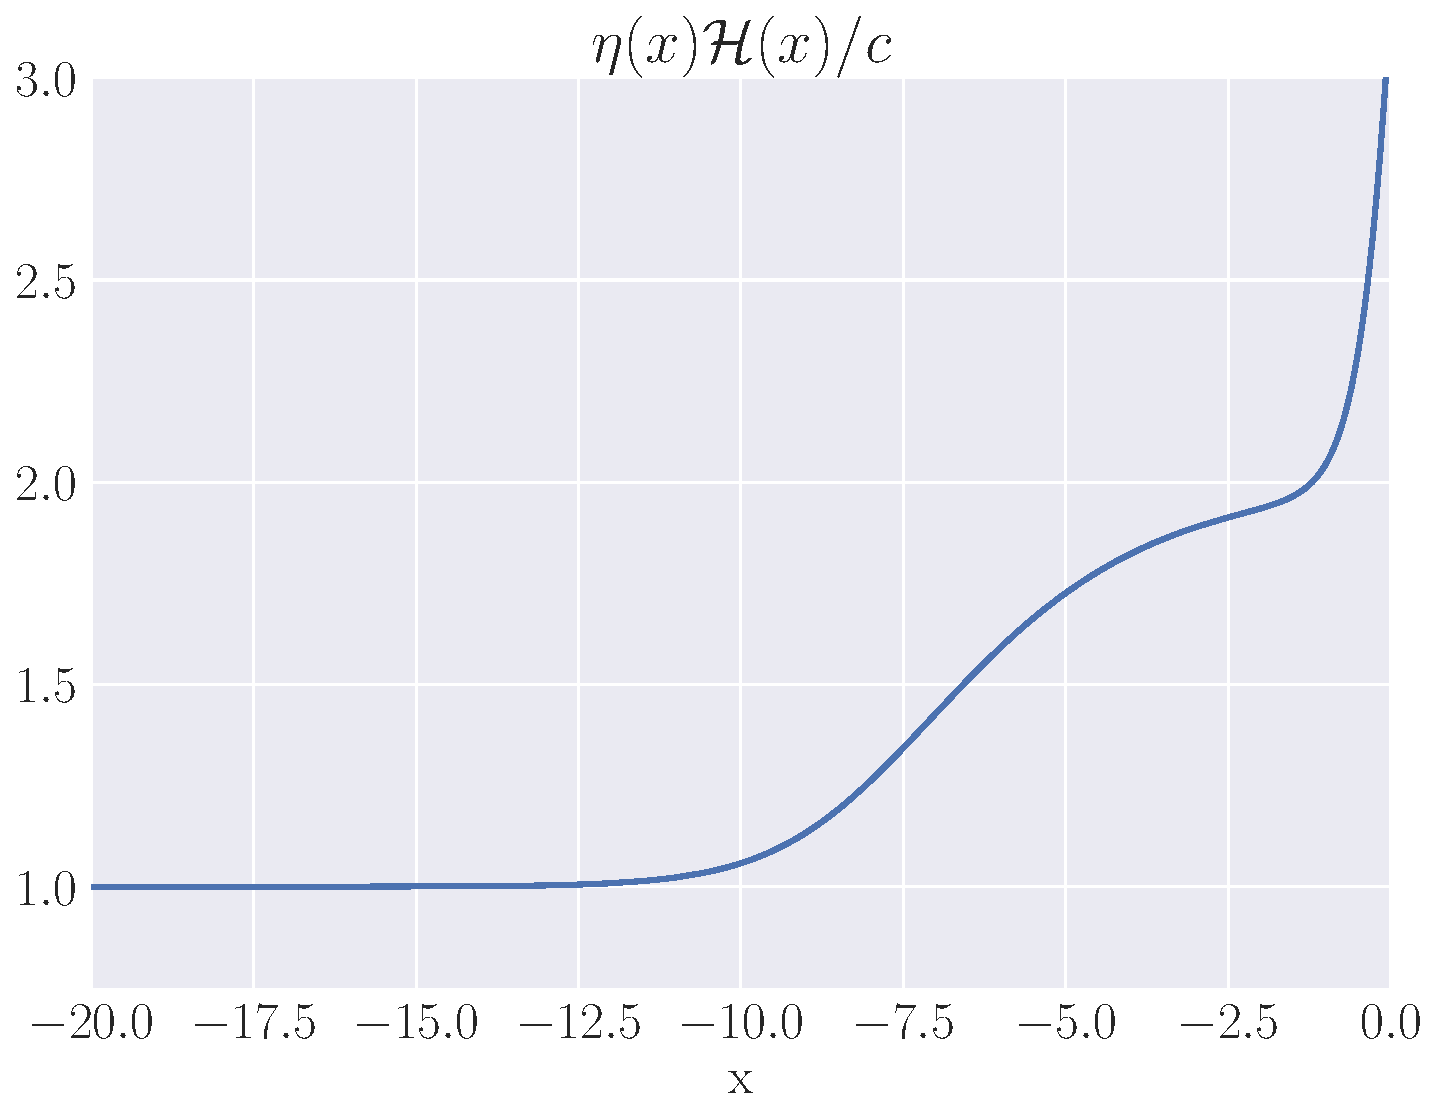
\includegraphics[width=\linewidth]{compare_eta_H_over_c.pdf}
    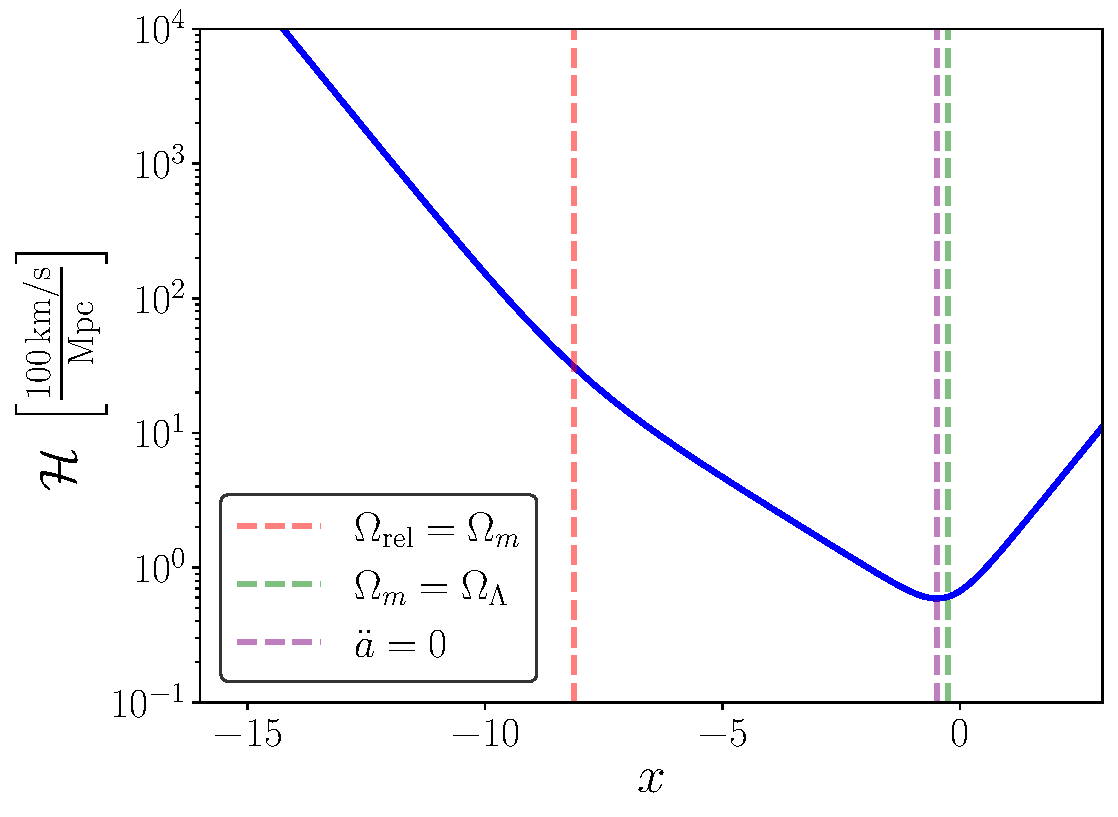
\includegraphics[width=\linewidth]{compare_Hp.pdf}
\end{figure}

\begin{figure}[ht!]
    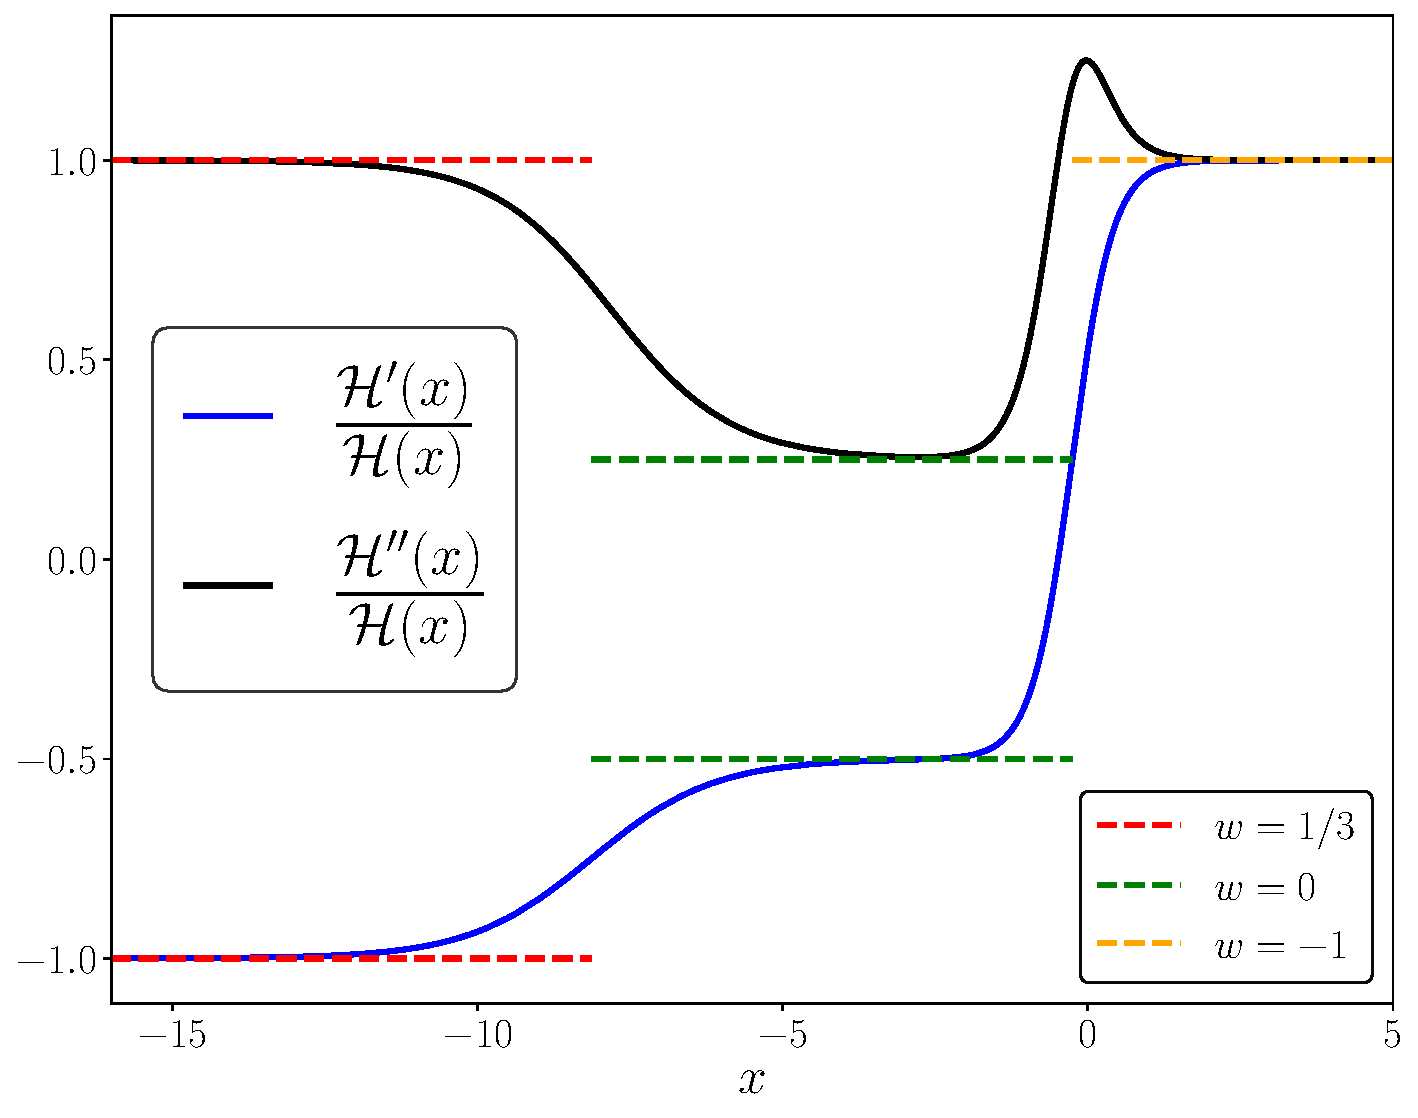
\includegraphics[width=\linewidth]{dH_and_ddH_over_H.pdf}
\end{figure}

\begin{figure}[ht!]
    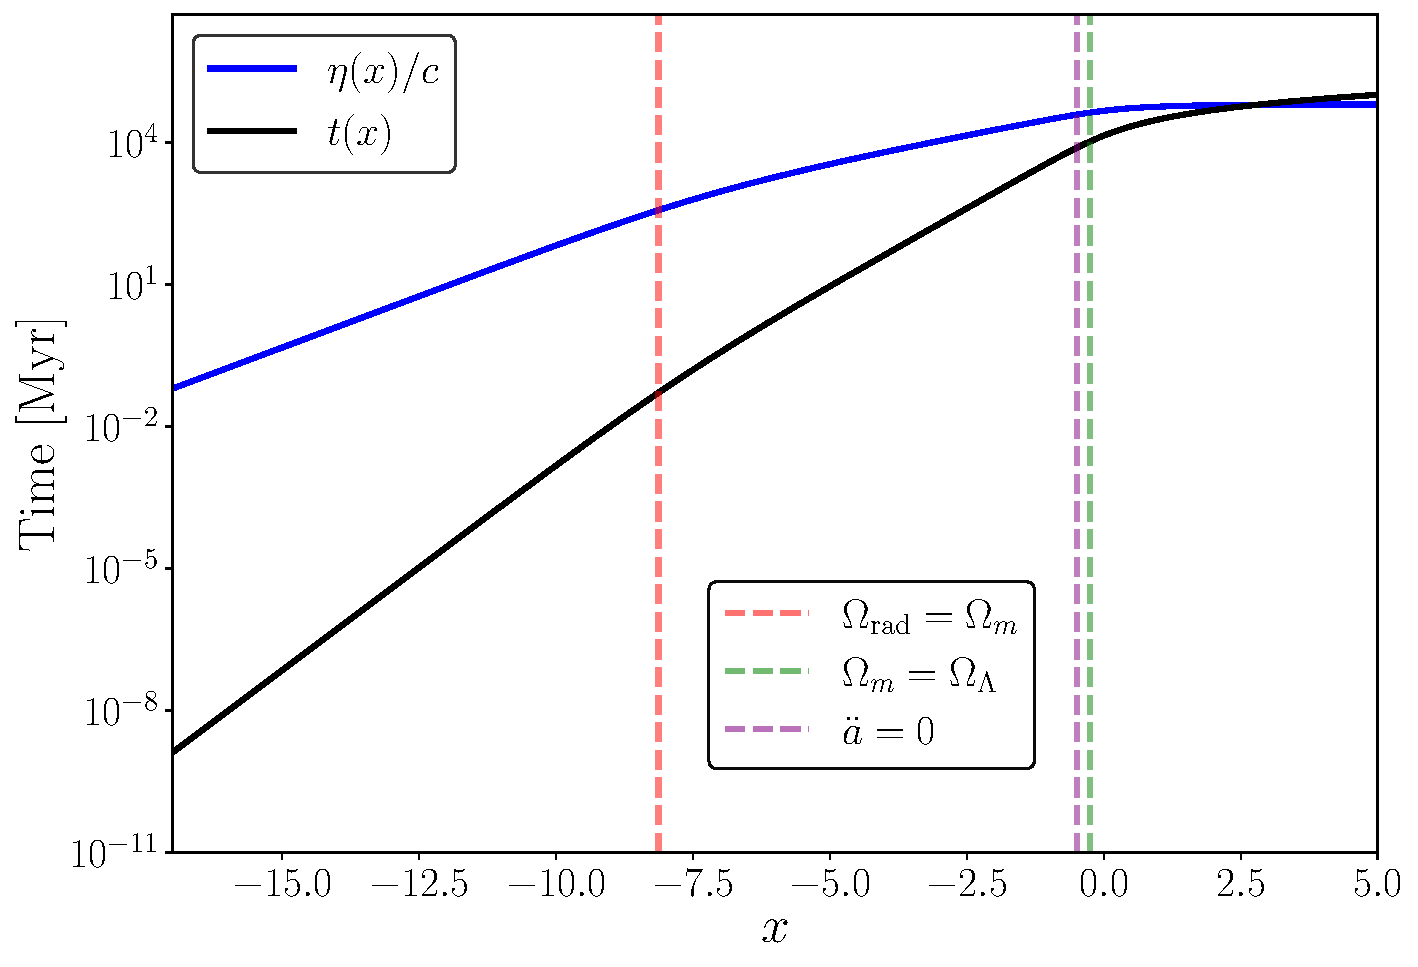
\includegraphics[width=\linewidth]{t_and_eta_c.pdf} 
\end{figure}


\begin{figure}[ht!]
    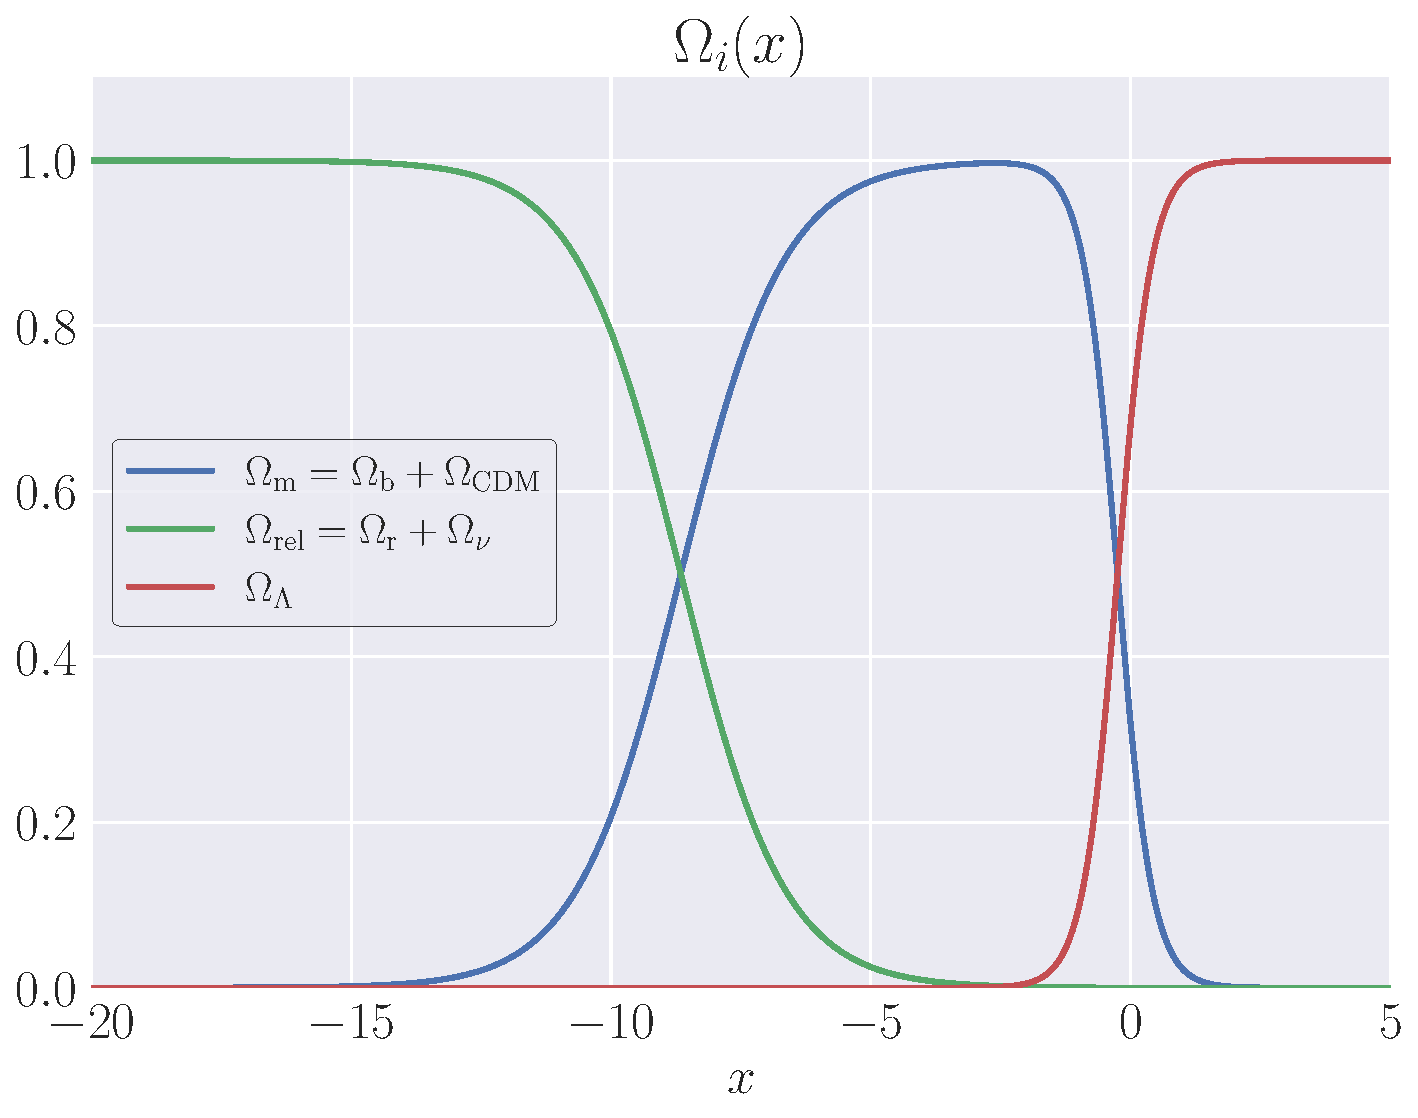
\includegraphics[width=\linewidth]{omega_i_of_x.pdf}
\end{figure}

\begin{figure}[ht!]
    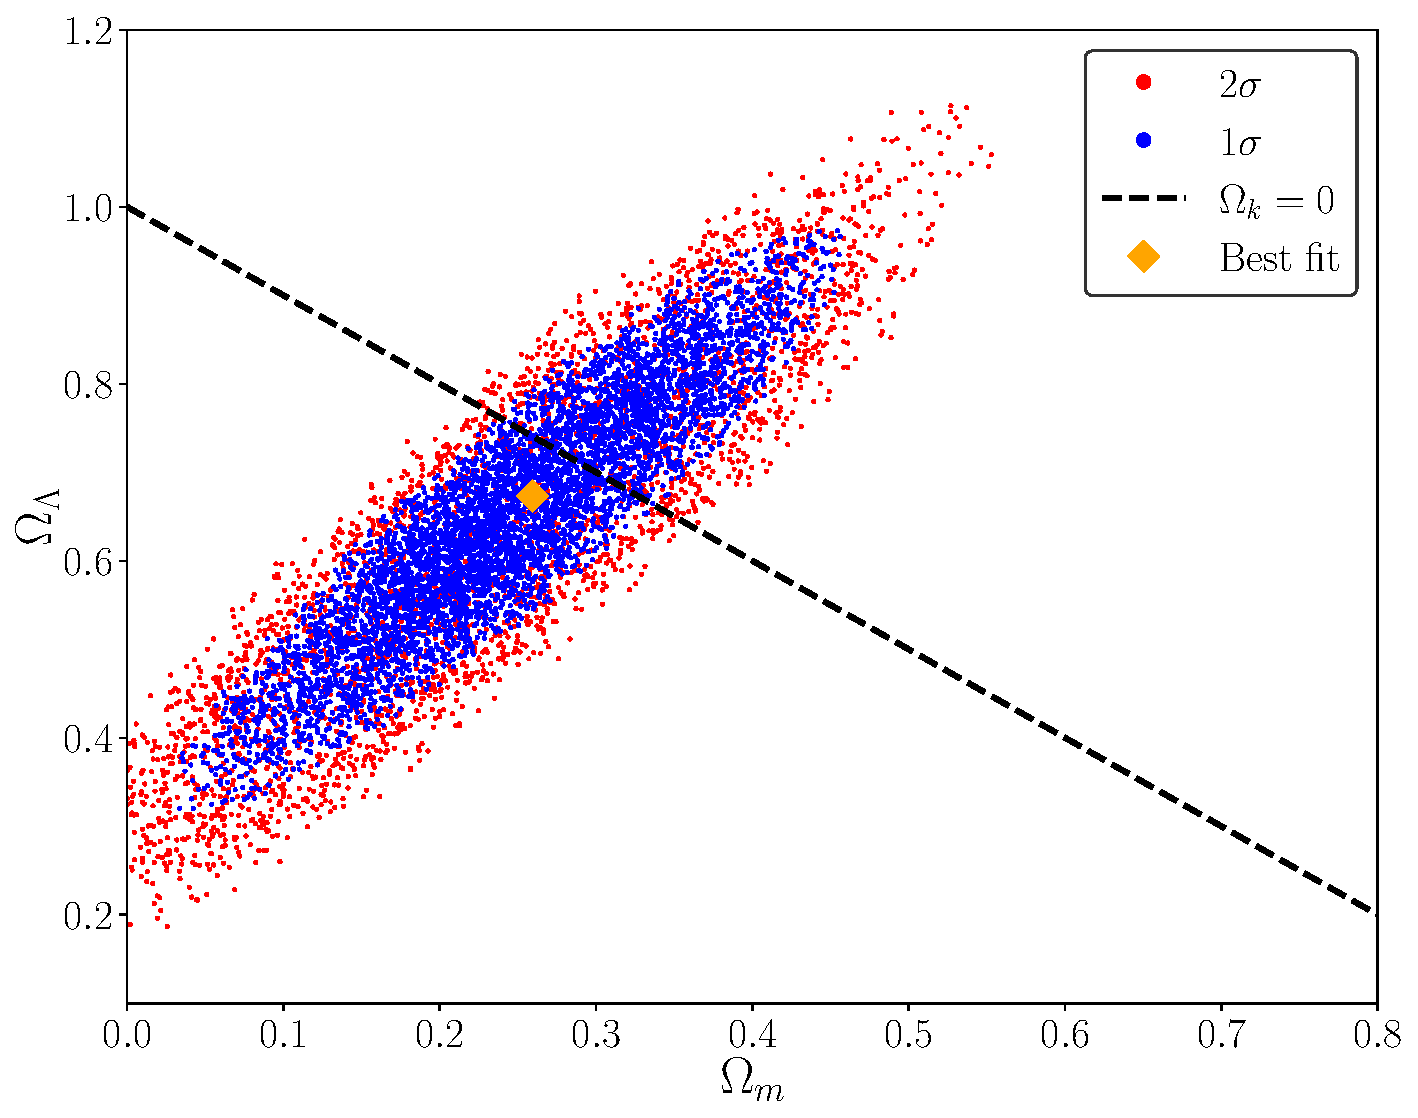
\includegraphics[width=\linewidth]{mcmc_supernova_fit_Nburn1000.pdf}
    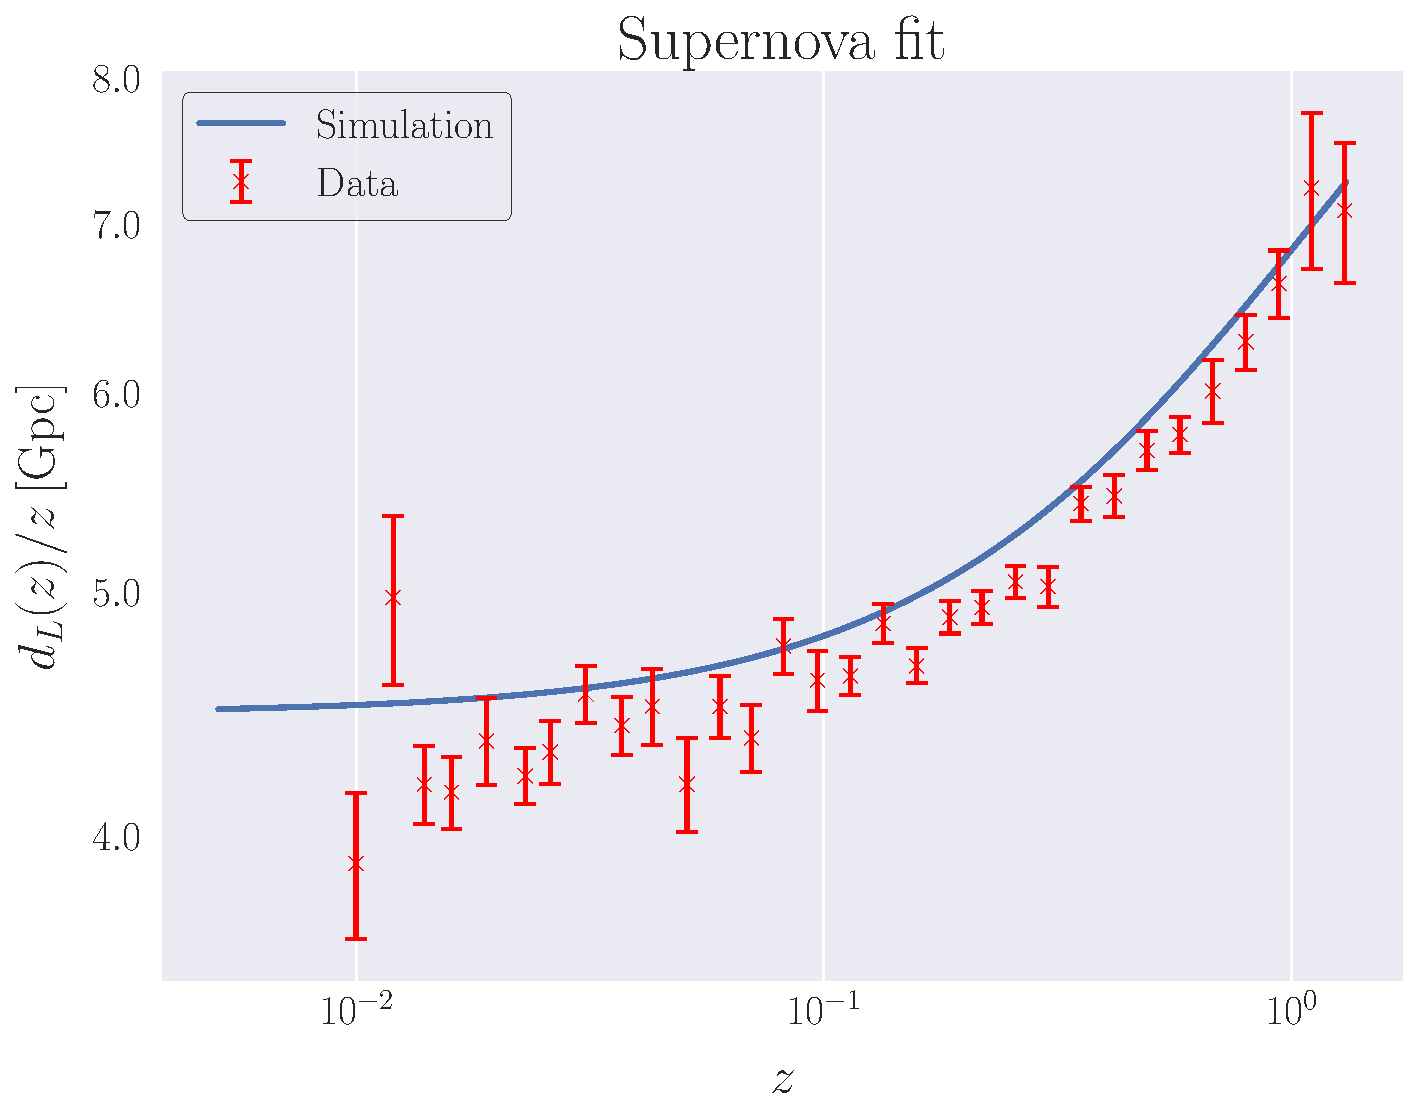
\includegraphics[width=\linewidth]{dL_z_compare_log.pdf}
\end{figure}

\begin{figure}[ht!]
    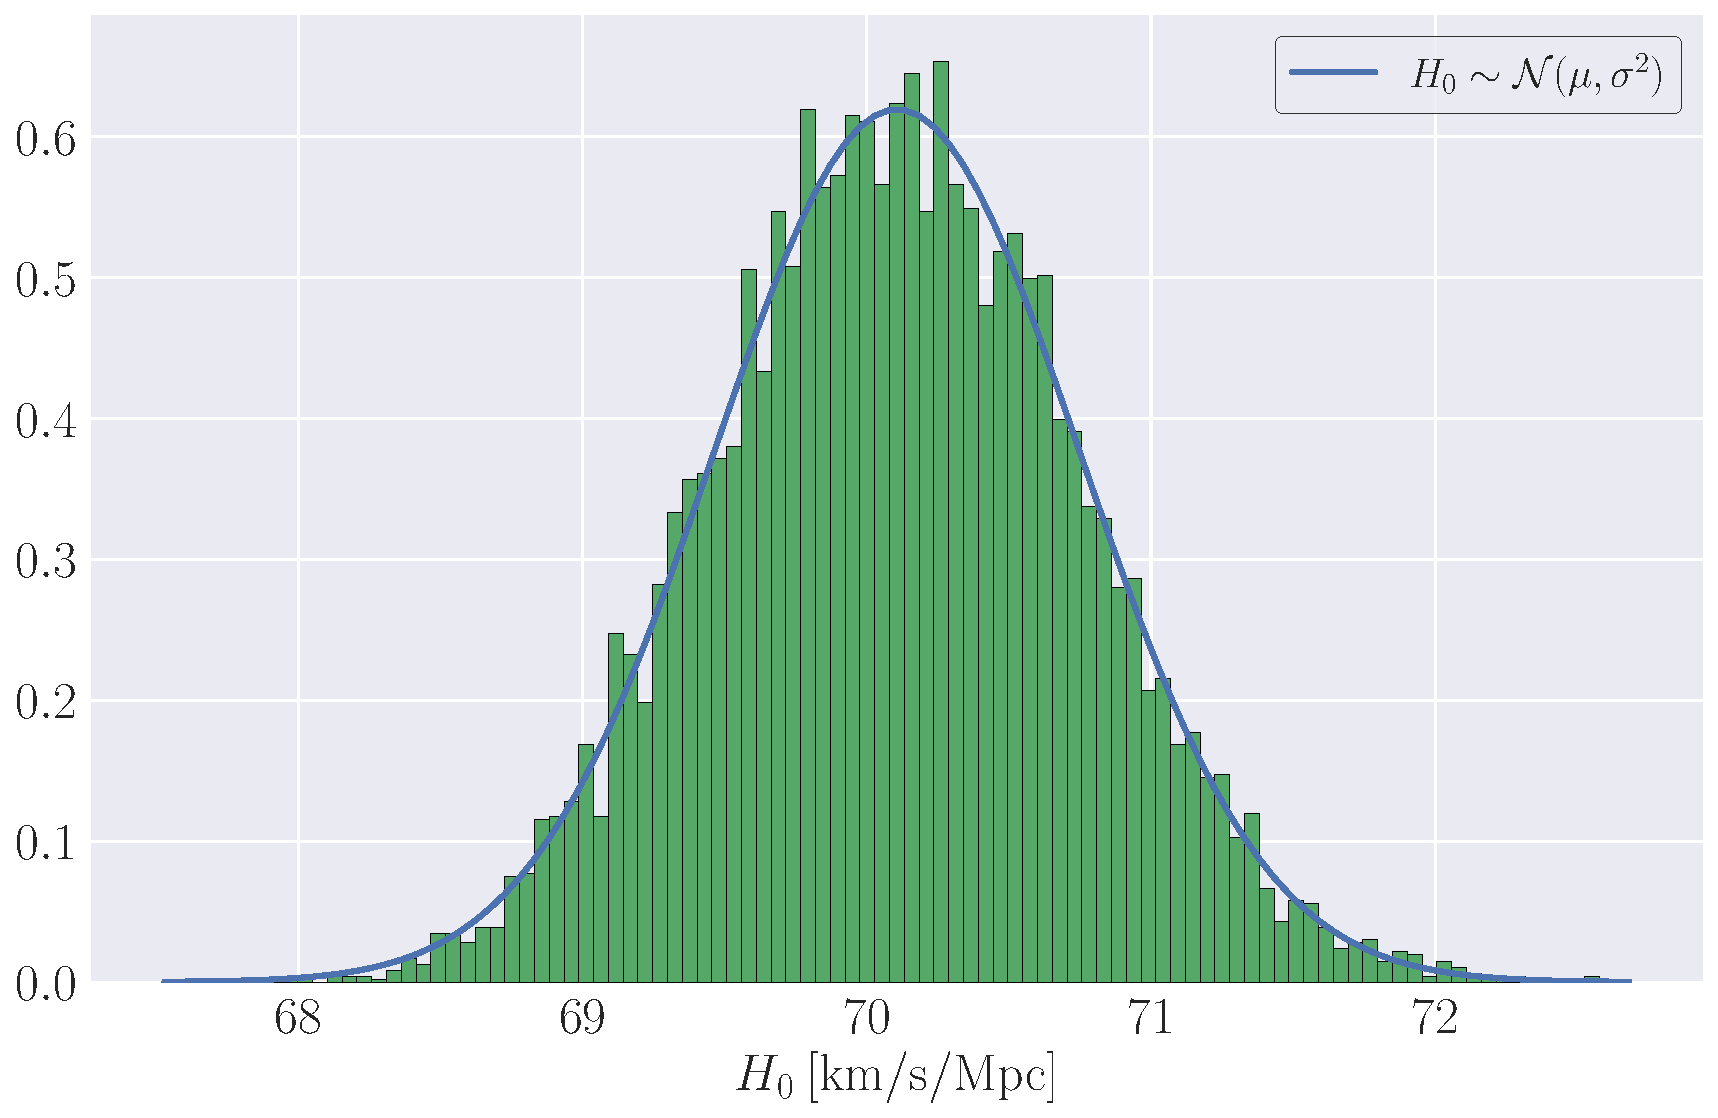
\includegraphics[width=\linewidth]{H0_pdf_Nburn1000.pdf}    
\end{figure}